\documentclass{standalone}
\usepackage{tikz}
\usepackage{ctex,siunitx}
\setCJKmainfont{Noto Serif CJK SC}
\usepackage{tkz-euclide}
\usepackage{amsmath}
\usepackage{wasysym}
\usetikzlibrary{patterns, calc}
\usetikzlibrary {decorations.pathmorphing, decorations.pathreplacing, decorations.shapes,}
\begin{document}
\small
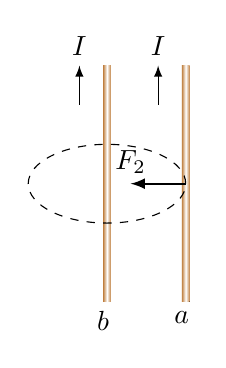
\begin{tikzpicture}[>=latex,scale=1]
  \foreach \x/\y in {0.1/b,1.1/a}
  {
    \fill[left color=brown,right color=brown,middle color=white](\x-0.05,0.5)rectangle(\x+0.05,3.5)node[at start,below]{$\y$};
  }
  \draw[dashed] (.1,2) ellipse [x radius = 1, y radius =.5];
  \draw [->](-.25, 3)--(-.25, 3.5)node[above]{$I$};
  \draw[->] (.75, 3)--(.75, 3.5)node[above]{$I$};
  \draw[->,thick] (1.1,2)--(.4,2)node[above]{$F_2$};
\end{tikzpicture}
\end{document}